\section{Planung für die 2. Phase: Experiment}
Die Aspekte, welche in \textit{3. Sicherheitsrisiken} und \textit{4. Schutzmechanism} beschrieben wurden, sollen anhand
eines Expirementes verdeutlicht werden. Mithilfe eines selbstgebauten IoT-Gerätes sollen potentielle Sicherheitsrisken, 
welche ein Angreifer ausnutzen kann, sowie Schutzmechanism, um diesen entgegenzuwirken, vorgestellt und erklärt werden.

\subsection{Sicherheitskamera}
Das IoT-Geräte, welches für das Experiment entwickelt werden soll, ist eine Sicherheitskamera, die mithilfe der Kamera
einen Bereich überwacht und dessen Bilderaufnahmen von  weiteren System aufgerufen werden können. \\

Die Sicherheitskamera soll mit einem \textit{Raspberry PI} und einem Kamera-Adapter umgesetzt werden.
Die Bilderaufnahmen, die von der Kamera erstellt werden, sollen über ein Programm ausgelesen und über
einen auf dem \textit{Raspberry PI} laufenden Server abrufbar sein. \\

	\begin{figure}[h]
		\centering
		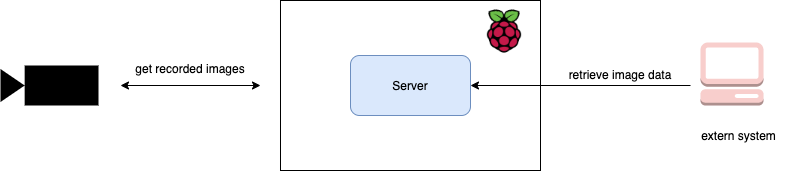
\includegraphics[width=145mm]{images/raspberrypi.png}
		\caption{Sicherheitskamera-Architektur}
		\label{fig:arch-raspberrypi}
	\end{figure}
